\chapter{Исследовательская часть}

В данном разделе будут приведены примеры работы программы, и будет проведен сравнительный анализ реализованных алгоритмов поиска редакционного расстояния по затраченному процессорному времени.

\section{Технические характеристики}

Тестирование проводилось на устройстве со следующими техническими характеристиками:

\begin{itemize}
	\item операционная система: Ubuntu 20.04.1 Linux x86\_64 \cite{linux};
	\item память : 8 GiB;
	\item процессор: AMD® Ryzen™ 3 3200u @ 2.6 GHz \cite{amd}.
\end{itemize}

Тестирование проводилось на ноутбуке, включенном в сеть электропитания. Во время тестирования ноутбук был нагружен только встроенными приложениями окружения, а также непосредственно системой тестирования.

\clearpage

\section{Демонстрация работы программы}

На рисунке \ref{img:example} приведен пример работы программы.

\begin{figure}[H]
	\begin{center}
		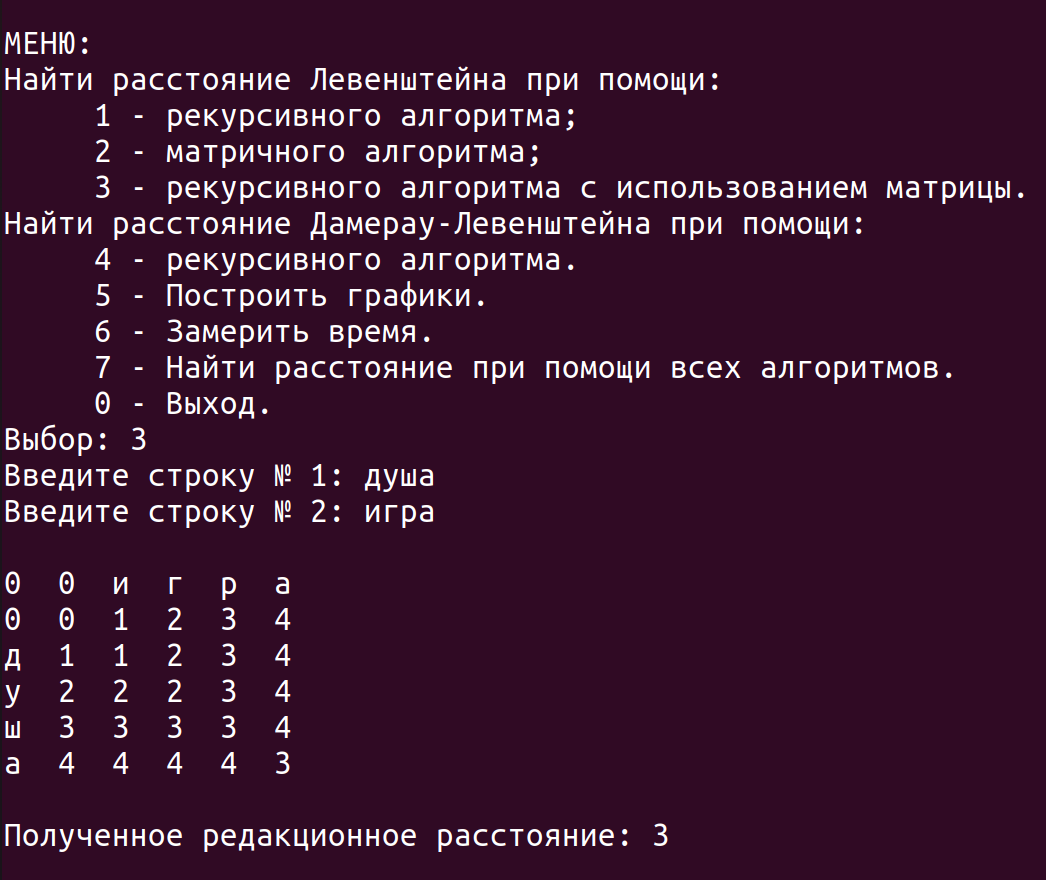
\includegraphics[scale=0.4]{img/example.png}
	\end{center}
	\captionsetup{justification=centering}
	\caption{Пример работы программы}
	\label{img:example}
\end{figure}

\section{Время выполнения алгоритмов}

Функция process\_time из библиотеки time ЯП Python возвращает  процессорное время в секундах - значение типа float.

Для замера времени:
\begin{itemize}
	\item получить значение времени до начала выполнения алгоритма, затем после её окончания. Чтобы получить результат, необходимо вычесть из второго значения первое;
	\item первый шаг необходимо повторить iters раз (в программе iters равно 100), суммируя полученные значения, а затем усреднить результат.
\end{itemize}

Замеры проводились для длины слов от 0 до 8 на случайных входных строках. Результаты измерения времени приведены в таблице \ref{tbl:time_mes} (в мс).

\begin{table}[h]
    \begin{center}
        \begin{threeparttable}
        \captionsetup{justification=raggedright,singlelinecheck=off}
        \caption{Результаты замеров времени}
        \label{tbl:time_mes}
        \begin{tabular}{|c|c|c|c|c|}
            \hline
            Длина & Рек-ый (Л.) & Матр-ый & Рек-ый с кэшем & Рек-ый (Д.-Л.)  \\
            \hline
    			0 & 0.0022 & 0.0053 & 0.0019 & 0.0010 \\ 
 			\hline
    			1 & 0.0062 & 0.0073 & 0.0047 & 0.0029 \\ 
 			\hline
    			2 & 0.0214 & 0.0130 & 0.0076 & 0.0112 \\ 
 			\hline
    			3 & 0.0645 & 0.0198 & 0.0148 & 0.0469 \\ 
 			\hline
    			4 & 0.1988 & 0.0263 & 0.0223 & 0.2364 \\ 
 			\hline
    			5 & 1.0346 & 0.0458 & 0.0320 & 1.2427 \\ 
 			\hline
    			6 & 5.4673 & 0.0290 & 0.0423 & 7.0460 \\ 
 			\hline
    			7 & 35.5647 & 0.0331 & 0.0639 & 39.0492 \\ 
 			\hline
    			8 & 189.6622 & 0.0419 & 0.0729 & 199.8746 \\ 
			\hline
		\end{tabular}
    \end{threeparttable}
\end{center}
\end{table}

На рисунках \ref{img:first}-\ref{img:third} приведены графические результаты сравнения временных характеристик.

\begin{figure}[H]
	\begin{center}
		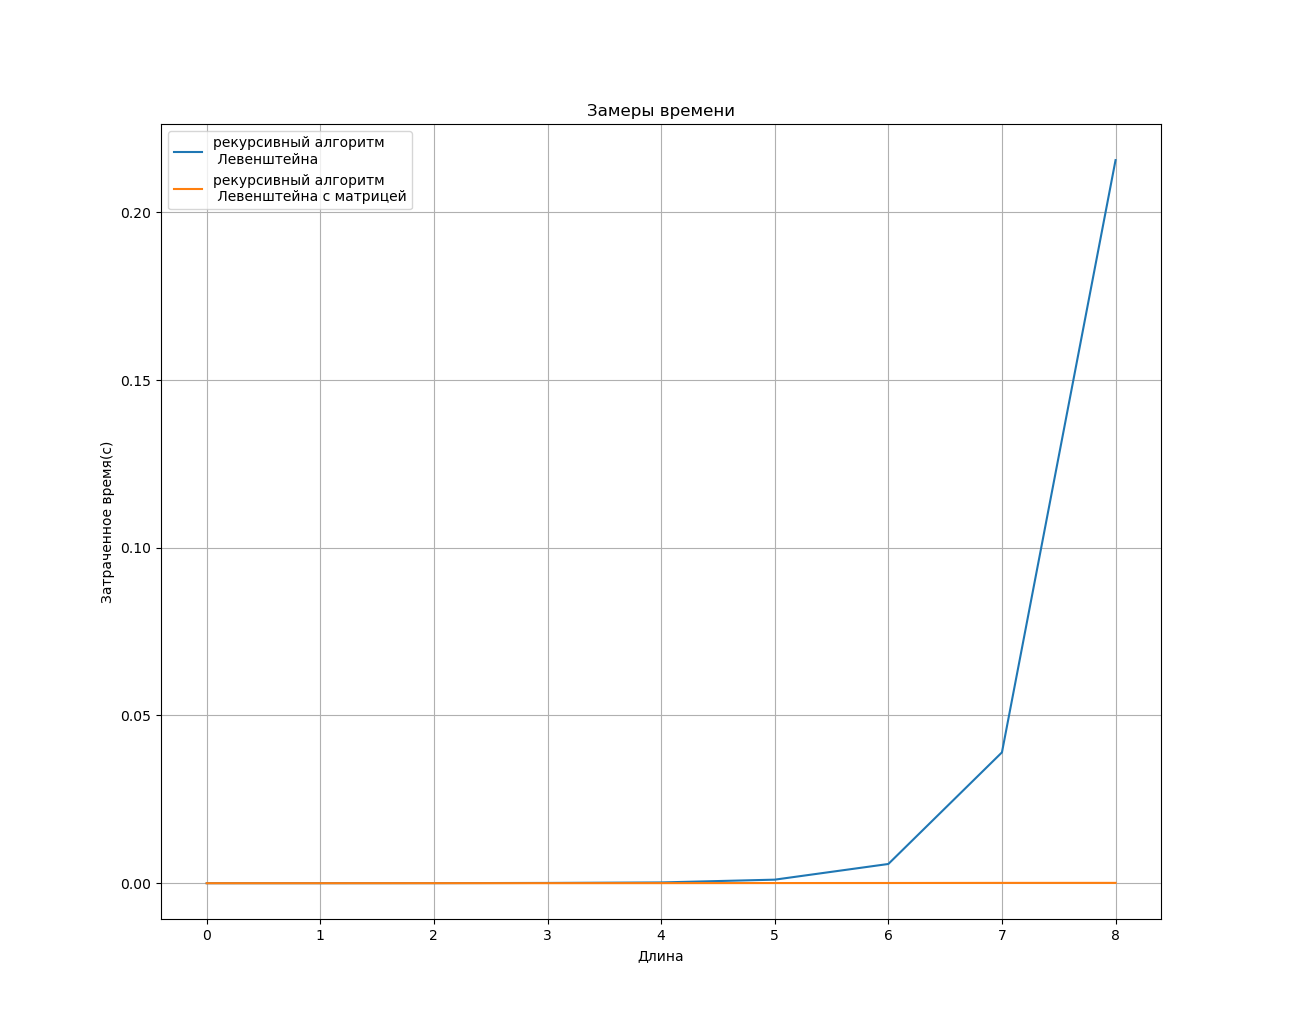
\includegraphics[scale=0.5]{img/first.png}
	\end{center}
	\captionsetup{justification=centering}
	\caption{Сравнение по времени рекурсивного алгоритма Левенштейна и рекурсивного алгоритма Левенштейна с использованием кэша}
	\label{img:first}
\end{figure}

\begin{figure}[H]
	\begin{center}
		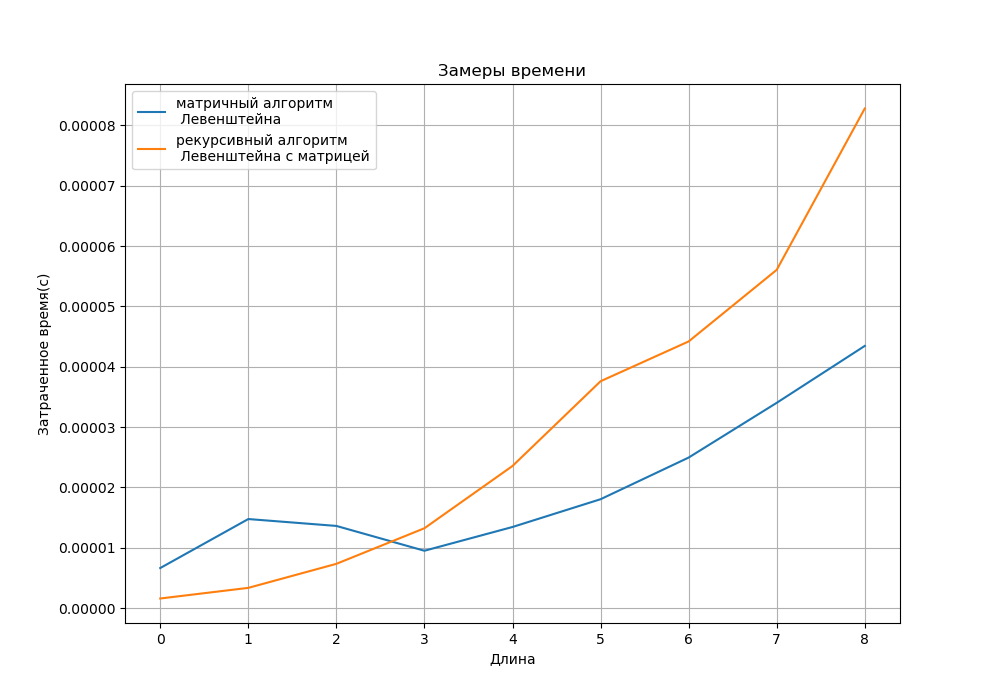
\includegraphics[scale=0.6]{img/second.png}
	\end{center}
	\captionsetup{justification=centering}
	\caption{Сравнение по времени матричного алгоритма Левенштейна и алгоритма Левенштейна с использованием кэша}
	\label{img:second}
\end{figure}

\begin{figure}[H]
	\begin{center}
		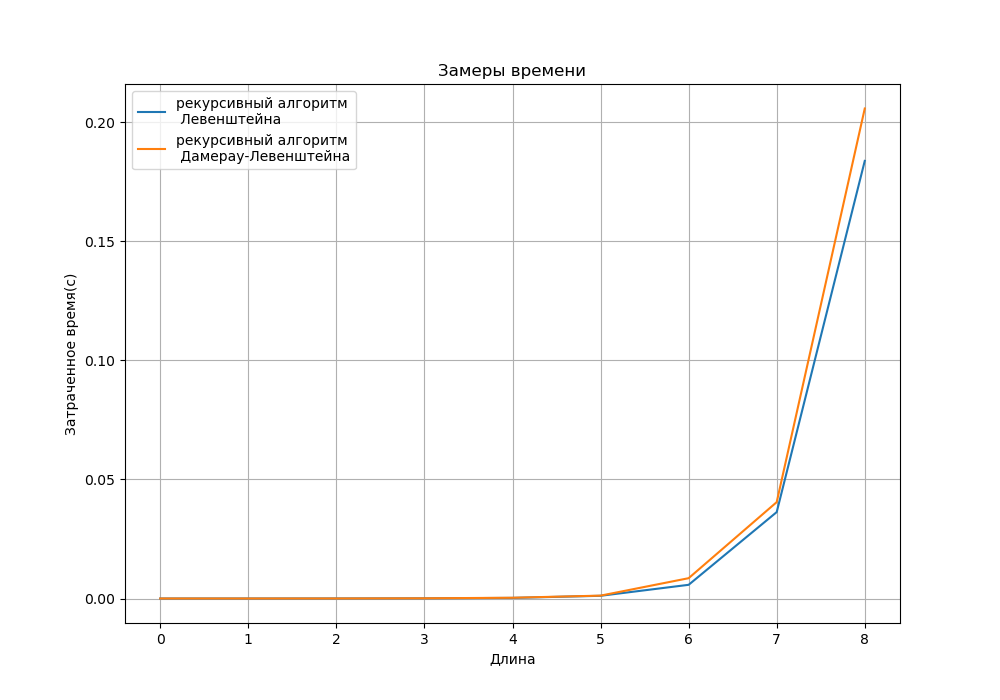
\includegraphics[scale=0.6]{img/third.png}
	\end{center}
	\captionsetup{justification=centering}
	\caption{Сравнение по времени рекурсивного алгоритма Левенштейна и рекурсивного алгоритма Дамерау-Левенштейна}
	\label{img:third}
\end{figure}

\section{Вывод}

Исходя из замеров по памяти, итеративные алгоритмы проигрывают рекурсивным, потому что максимальный размер памяти в них растет, как произведение длин строк, а в рекурсивных - как сумма длин строк.

В результате эксперимента было получено, что при длине строк в 4 символа, рекурсивная реализация алгоритма Левенштейна становится медленнее матричной в 9 раз и с увеличением длины строк время работы растет в геометрической прогрессии. Тогда, для строк длиной более 4 символов небходимо использовать матричную версию алгоритма поиска редакционного расстояния.

Также в результате эксперимента было установлено, что при длине строк в более 5 символов, алгоритм Левенштейна работает быстрее Дамерау-Левенштейна в 1.3 раза. Можно сделать вывод, что при таких данных предпочтительно использовать алгоритм Левенштейна.